%! TEX root = **/010-main.tex
% vim: spell spelllang=en:

\section{Comparison}%
\label{sec:comparison}

% Comparison and discussion of results of the different data mining methods on the validation data-set.
% Which is the best method when testing on the validation data set?  Write a comparative table.
% Try to compare different methods using McNemar test or at least show the interval of confidence for each method.
% Is there an explanation for those results (some hypothesis applicable,  etc.)? 
% Are in general accuracy on validation data set similar to the obtained with cross-validation?   
% Are  there  for  some  methods  huge  differences? If  that’s  the  case,why do you think that happens?
% Final personal evaluation of which is the best method you consider and why.

Once we have all the algorithms implemented we are going to compare them to find out which yields the best results in our dataset. To do so we run the algorithms with their respective best parameters on the testing dataset and we get the following table:

\begin{table}[H]
\centering
\caption{Comparison of metrics}%
\label{tab:comparison}
\begin{tabular}{lrr}
\toprule
{} &  Accuracy &        F1 \\
\midrule
nb     &  0.871667 &  0.813559 \\
knn    &  0.856667 &  0.788177 \\
dt     &  0.910000 &  0.858639 \\
svm    &  0.911667 &  0.865140 \\
voting &  0.908333 &  0.858612 \\
bag    &  0.925000 &  0.882507 \\
rf     &  0.925000 &  0.881890 \\
ada    &  0.923333 &  0.881443 \\
\bottomrule
\end{tabular}

\end{table}

Looking at \cref{tab:comparison} we can see that meta learning algorithms have the best f1-scores and accuracies. Bagging is tied with random forests for the best accuracy but it has a slightly higher f1-score. Another thing to point out is that knn is the worse performing algorithm. Despite all of this all the algorithms have relatively similar results, we only have a 0.4\% accuracy and a 0.5\% f1-score difference between the best and worst. 

Next we continue the comparison by performing chi-squared mcNemar tests among all algorithms to find out whether or not there is a meaningful difference between them.

\begin{figure}[H]
\centering
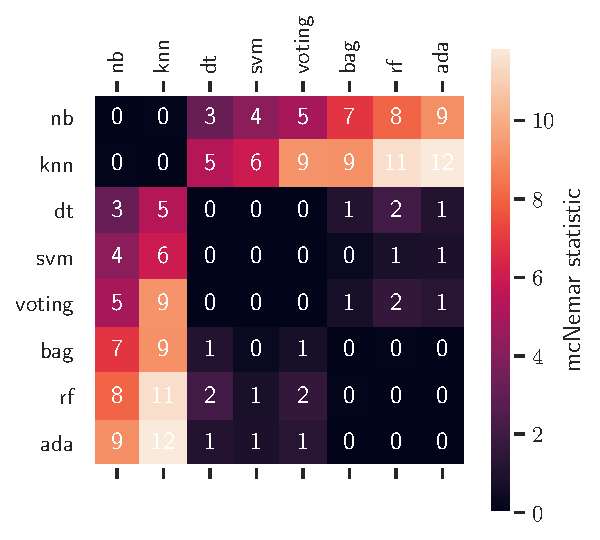
\includegraphics{chi_mcnemar}
\caption{mcNemar statistic}
\end{figure}

\begin{figure}[H]
\centering
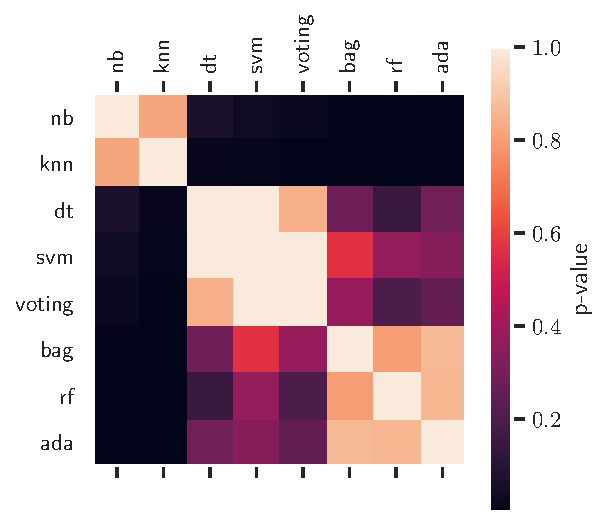
\includegraphics{chi_mcnemar_pvalue}
\caption{mcNemar test $p$-value}
\end{figure}

\begin{table}[H]
\centering
\caption{mcNemar test $p$-values}
\label{tab:p-values}
\begin{tabular}{lrrrrrrrr}
\toprule
{} &   nb &  knn &   dt &  svm &  voting &  bag &   rf &  ada \\
\midrule
nb     & 1.00 & 0.42 & 0.01 & 0.00 &    0.00 & 0.00 & 0.00 & 0.00 \\
knn    & 0.42 & 1.00 & 0.00 & 0.00 &    0.00 & 0.00 & 0.00 & 0.00 \\
dt     & 0.01 & 0.00 & 1.00 & 1.00 &    1.00 & 0.09 & 0.09 & 0.29 \\
svm    & 0.00 & 0.00 & 1.00 & 1.00 &    0.88 & 0.30 & 0.30 & 0.34 \\
voting & 0.00 & 0.00 & 1.00 & 0.88 &    1.00 & 0.11 & 0.12 & 0.22 \\
bag    & 0.00 & 0.00 & 0.09 & 0.30 &    0.11 & 1.00 & 1.00 & 1.00 \\
rf     & 0.00 & 0.00 & 0.09 & 0.30 &    0.12 & 1.00 & 1.00 & 1.00 \\
ada    & 0.00 & 0.00 & 0.29 & 0.34 &    0.22 & 1.00 & 1.00 & 1.00 \\
\bottomrule
\end{tabular}

\end{table}

When analyzing the $p$-values obtained by the mcNemar test we want to have $95\%$ of confidence level, therefore we will set $\alpha = 0.05$. If we get $p > \alpha$ we fail to reject the $H0$. Otherwise if $p \leq \alpha$ we reject $H0$. When looking at \cref{tab:p-values} we can clearly see that Na\"ve Bayes and Knn have $p$-values smaller than alpha when tested against any other algorithm. Therefore we can reject H0 and conclude that they have significantly different performance than the rest. When analysing other algorithms we fail to reject the null hypothesis and therefore their performance is relatively similar. 

Na\"ive Bayes and Knn had the worst scoring results \cref{tab:comparison}. Therefore we end up concluding that choosing any of the other algorithms will give better results. As they aren't significantly different between them the choice to use one or the other depends individual preference and computational cost.